\documentclass[unicode,aspectratio=43]{beamer}
\usetheme{Moscow}

\usepackage[utf8]{inputenc}
\usepackage[T2A]{fontenc}
\usepackage[main=russian,english]{babel}

\usepackage{amsmath,amssymb}

\hypersetup{
	pdfauthor={Ivan Tsybulin}
}

%\renewcommand{\thefootnote}{\fnsymbol{footnote}}
\usepackage{euler}
\usepackage{multirow}
\renewcommand*{\arraystretch}{1.2}

\graphicspath{{images/}}
\newcommand{\colorhref}[2]{\href{#1}{\textcolor{miptbase!30!black}{#2}}}

\newcounter{citenum}
\newcommand{\newtotcounter}[1]{}
%%% Реализация библиографии встроенными средствами посредством движка bibtex8 %%%

%%% Пакеты %%%
\usepackage{cite}                                   % Красивые ссылки на литературу


%%% Стили %%%
\bibliographystyle{../BibTeX-Styles/utf8gost71umod}    % Оформляем библиографию по ГОСТ 7.1 (ГОСТ Р 7.0.11-2011, 5.6.7)

\makeatletter
\renewcommand{\@biblabel}[1]{#1.}   % Заменяем библиографию с квадратных скобок на точку
\makeatother
%% Управление отступами между записями
%% требует etoolbox 
%% http://tex.stackexchange.com/a/105642
%\patchcmd\thebibliography
% {\labelsep}
% {\labelsep\itemsep=5pt\parsep=0pt\relax}
% {}
% {\typeout{Couldn't patch the command}}

%%% Цитирование %%%
\renewcommand\citepunct{;\penalty\citepunctpenalty%
    \hskip.13emplus.1emminus.1em\relax}                % Разделение ; при перечислении ссылок (ГОСТ Р 7.0.5-2008)


%%% Создание команд для вывода списка литературы %%%
\newcommand*{\insertbibliofull}{
\bibliography{../biblio/othercites,../biblio/authorpapersVAK,../biblio/authorpapers,../biblio/authorconferences}         % Подключаем BibTeX-базы % После запятых не должно быть лишних пробелов — он "думает", что это тоже имя пути
}

\newcommand*{\insertbiblioauthor}{
\bibliography{../biblio/authorpapersVAK,../biblio/authorpapers,../biblio/authorconferences}         % Подключаем BibTeX-базы % После запятых не должно быть лишних пробелов — он "думает", что это тоже имя пути
}

\newcommand*{\insertbiblioother}{
\bibliography{../biblio/othercites}         % Подключаем BibTeX-базы
}


%% Счётчик использованных ссылок на литературу, обрабатывающий с учётом неоднократных ссылок
%% Требуется дважды компилировать, поскольку ему нужно считать актуальный внешний файл со списком литературы
\newtotcounter{citenum}
\def\oldcite{}
\let\oldcite=\bibcite
\def\bibcite{\stepcounter{citenum}\oldcite}

\renewcommand{\citepunct}{,\,}

\title[Численные методы решения УПИ]{Разработка численных методов для решения уравнения переноса излучения и их реализация с использованием графических ускорителей}
\date{15 октября 2015, МФТИ, Москва}
\author[Цыбулин Иван]{\textbf{Цыбулин Иван}\\[1ex]
Специальность 05.13.18 -- Математическое моделирование, численные методы и
комплексы программ\\[1ex]
Научный руководитель:\\
кандидат физико-математических наук,\\
\textbf{Скалько Юрий Иванович}}
\institute[МФТИ]{Московский физико-технический институт}

\newcommand{\I}{\mathrm{\mathit{I}}}
\newcommand{\Ip}{\mathrm{\mathit{I}}_\text{p}}
\renewcommand{\vec}[1]{\boldsymbol{\mathbf{#1}}}
\newcommand{\pd}[2]{\frac{\partial #1}{\partial #2}}
\let\dividesymbol\div
\renewcommand{\div}{\operatorname{div}}
\newcommand{\grad}{\operatorname{grad}}

\begin{document}
\begin{frame}[plain]
\maketitle
\end{frame}

\begin{frame}[plain]
\footnotesize
\tableofcontents
\end{frame}

\section{Введение}

\subsection{Общая характеристика работы}

\begin{frame}\frametitle{Актуальность}
	Задачи, в которых излучение существенно:
	\begin{itemize}
	\item Сильноточные разряды в установках на основе пинч-эффекта --- мощные источники излучения.
	\item Моделирование астрофизических объектов --- аккреционных дисков, квазаров, релятивистских струй, и т. п.
	\item Моделирование климата планеты --- ключевая роль в атмосферном теплообмене.
	\end{itemize}
\end{frame}

\begin{frame}\frametitle{Степень разработанности}
	Для уравнения переноса излучения разработаны методы, учитывающие
	\begin{itemize}
	\item симметрию (плоская, цилиндрическая, сферическая);
	\item различные свойства коэффициента поглощения (приближение серой материи, оптически тонкого и оптически толстого слоя);
	\item приближенные способы описание углового распределения (приближение <<вперед-назад>>, диффузионное приближение);
	\item локализацию источников (дискретизация <<от границы>>).
	\end{itemize}
\end{frame}

\begin{frame}\frametitle{Цели работы}
	\begin{itemize}
	\item Построение и исследование численных методов решения уравнения переноса излучения.
	\item Реализация полученных методов с использованием графических ускорителей.
	\item Моделирование спектра линии H-$\alpha$ в излучении звезды Т Тельца при наличии конического ветра.
	\end{itemize}
\end{frame}

\begin{frame}\frametitle{Научная новизна}
	\begin{itemize}
	\item Впервые предложен вариационный метод для решения самосопряженного уравнения переноса излучения с базисом из радиальных угловых функций.
	\item Впервые предложен маршевый алгоритм для решения уравнения переноса на неструктурированной тетраэдральной сетке.
	\item Предложена оригинальная распределенная многопроцессорная реализация метода длинных характеристик.
	\end{itemize}
\end{frame}

\subsection{Уравнение переноса излучения}

\begin{frame}\frametitle{Постановка задачи}
	\begin{itemize}
	\item Поле излучения можно описать функцией интенсивности излучения $\I_\nu(\vec r,
\vec \Omega, t)$.
	\item В стационарном приближении интенсивность излучения не зависит от времени явно и
удовлетворяет уравнению переноса
	\[
		(\vec \Omega \nabla) \I_\nu + \varkappa_\nu \I_\nu = \varkappa_\nu \I_{\nu\text{p}},
	\]
	где $\varkappa_\nu(\vec r, \vec \Omega)$ --- коэффициент поглощения излучения в точке $\vec
r$, $\I_{\nu\text{p}}(\vec r, \vec \Omega)$ --- интенсивность равновесного излучения в точке.
	\item Граничные условия задают отсутствие источников излучения извне
области $G$:
	\[
		\I(\vec x, \vec \Omega) = 0, \qquad (\vec \Omega, \vec n) < 0, \quad
\vec x \in \partial G.
	\]
	\end{itemize}
\end{frame}

\begin{frame}\frametitle{Излучение в системе уравнений РГД}
	Для большинства задач радиационной газовой динамики достаточно учитывать только поток энергии, переносимый излучением. При этом плотностью энергии и импульсом излучения можно пренебречь.
	\[
	\begin{gathered}
	\pd{\rho}{t} + \div \rho \vec u = 0\\
	\pd{\rho \vec u}{t} + \div \left(\rho \vec u \vec u + p \mathbb I\right) = 0\\
	\pd{e}{t} + \div \left((e + p)\vec u + \vec S \right) = 0\\
	e = \rho \left(\varepsilon + \frac{u^2}{2}\right),\quad  p = p(\rho, \varepsilon),
	\end{gathered}
	\]

	Поток энергии излучения определяется как
	\[
	\vec S = \int_0^\infty \vec S_\nu d\nu \qquad\qquad
	\vec S_\nu = \int\limits_{4\pi} \I_\nu \vec \Omega d\Omega.
	\]
\end{frame}

\begin{frame}\frametitle{Вариационный принцип Владимирова}
	Четная по $\vec \Omega$ часть интенсивности излучения
	\[
	\varphi(\vec r, \vec \Omega) = \frac{\I(\vec r, \vec \Omega) + \I(\vec r, -\vec \Omega)}{2}
	\]
	доставляет минимум функционалу
	\[
	\mathcal{G}(\varphi) = [\varphi, \varphi] - 2(\varphi, \Ip) \to \min_{\varphi \in \mathfrak{H}_0},
	\]
	где
	\begin{align*}
	[u,v] &= (u, v) + \left(\frac{1}{\varkappa}(\vec \Omega \nabla) u, \frac{1}{\varkappa}(\vec \Omega \nabla) v\right)
	+ \iint\limits_{\partial G \times 4\pi} |\vec \Omega \vec n|uv d \vec r d\vec \Omega\\
	(u,v) &= \iint\limits_{\partial G \times 4\pi} \varkappa uv d \vec r d\vec
\Omega\\
	\mathfrak H_0 &= \Big\{\varphi(\vec r, \vec \Omega) \in H^{1}(G) \Big|
[\varphi, \varphi] < \infty\Big\}
	\end{align*}

\end{frame}

\section{Вариационный метод для УПИ}
\subsection{Дискретизация}
\begin{frame}\frametitle{Метод Ритца}
	Для дискретизации слабой постановки Владимирова использован метод Ритца. В качестве пространственного базиса выбраны кусочно-линейные функции:
	\[
	\varphi(\vec r, \vec \Omega) = \sum_{i= 1}^K \varphi_i(\vec r) \theta_i(\vec \Omega).
	\]
	\begin{columns}
	\begin{column}{.8\textwidth}
	В качестве углового базиса $\theta_i(\vec \Omega)$ рассмотрены
	\begin{itemize}
	\item сферические функции $Y_{2k,m}(\vec \Omega)$
	\item радиальные функции $R_i(\vec \Omega)$
	\end{itemize}
	\end{column}
	\begin{column}{.15\textwidth}
	\raggedleft 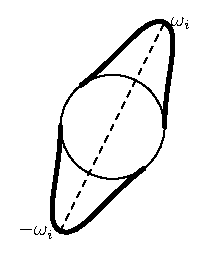
\includegraphics[width=\columnwidth]{rbf-0.eps}
	\end{column}
	\end{columns}
	\[
	R_i(\vec \Omega) = \exp\left(-\epsilon_i ||\vec \Omega - \vec \omega_i||^2\right) + \exp\left(-\epsilon_i ||\vec \Omega + \vec \omega_i||^2\right), \quad
	\epsilon_i = \frac{9\sqrt{3}}{8\gamma_i},
	\]
	где $\vec \omega_i, \gamma_i$ --- узлы и веса квадратурной формулы Лебедева для интегрирования по сфере.
\end{frame}	

\subsection{Решение системы линейных алгебраических уравнений}
\begin{frame}\frametitle{Блочно-диагональное предобуславливание}
    \begin{itemize}
    \item После пространственной дискретизации гармоник $\varphi_i(\vec r)$
    задача минимизации квадратичного функционала сводится к
    решению системы линейных алгебраических уравнений
    \item Для решения этой системы можно применить метод сопряженных градиентов с блочным проедобуславливателем Якоби.
    Каждый блок соответствует одной угловой гармонике.
    \item В терминах минимизации функционала предобуславливание
    соответствует решению совокупности задач минимизации для каждой гармоники в отдельности
    \[
        \varphi_i(\vec r) =
        \operatorname{\underset{\varphi_i}{\arg\min}} \mathcal{G}
\left[\varphi_i(\vec r) \theta_{i}(\vec \Omega) \right], \quad i = 1,\dots,K
    \]
	Данная задача эквивалентна решению набора скалярных эллиптических уравнений
вида
	\[
	-\div \left(\frac{1}{\varkappa} \mathbb D \grad \varphi\right) + \varkappa \varphi = f
	\]
    \end{itemize}
\end{frame}

\subsection{Результаты}

\begin{frame}\frametitle{Сходимость по угловой переменной}
Для тестовой задаче об излучающем оптически плотном шаре в оптически точкой среде исследовалась зависимость численного решения от числа используемых угловых функций
\begin{center}
	\only<1>{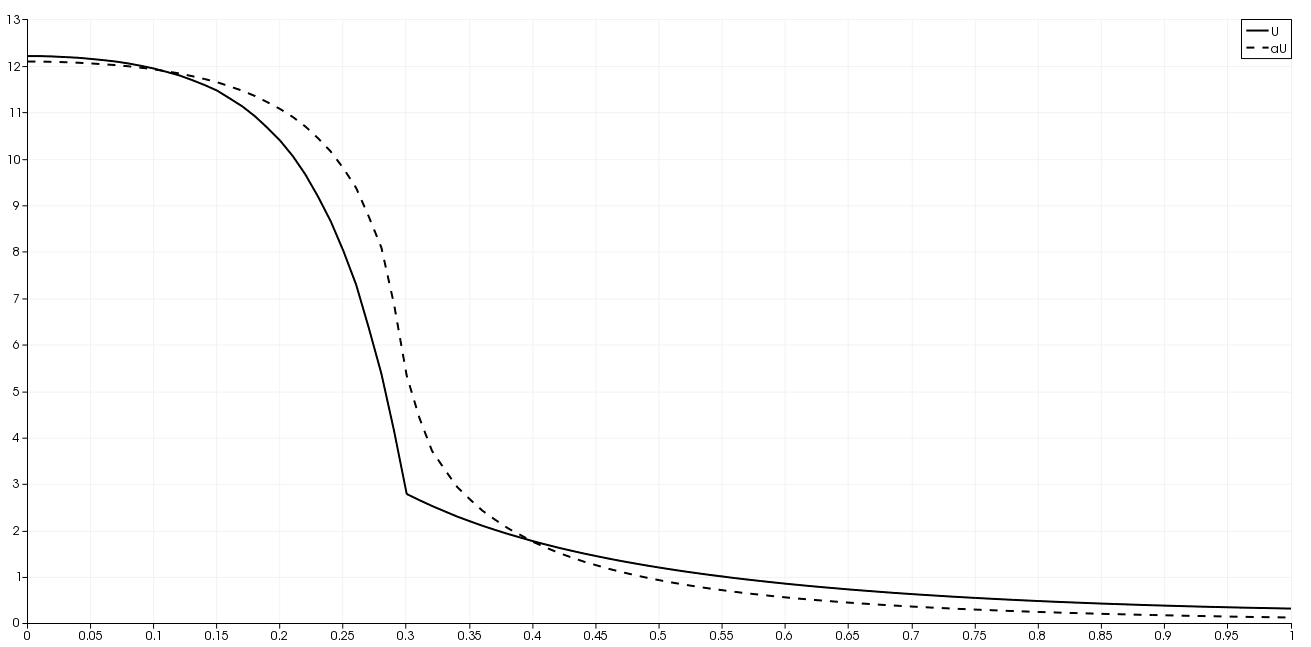
\includegraphics[height=0.5\textheight]{n1}}%
	\only<2>{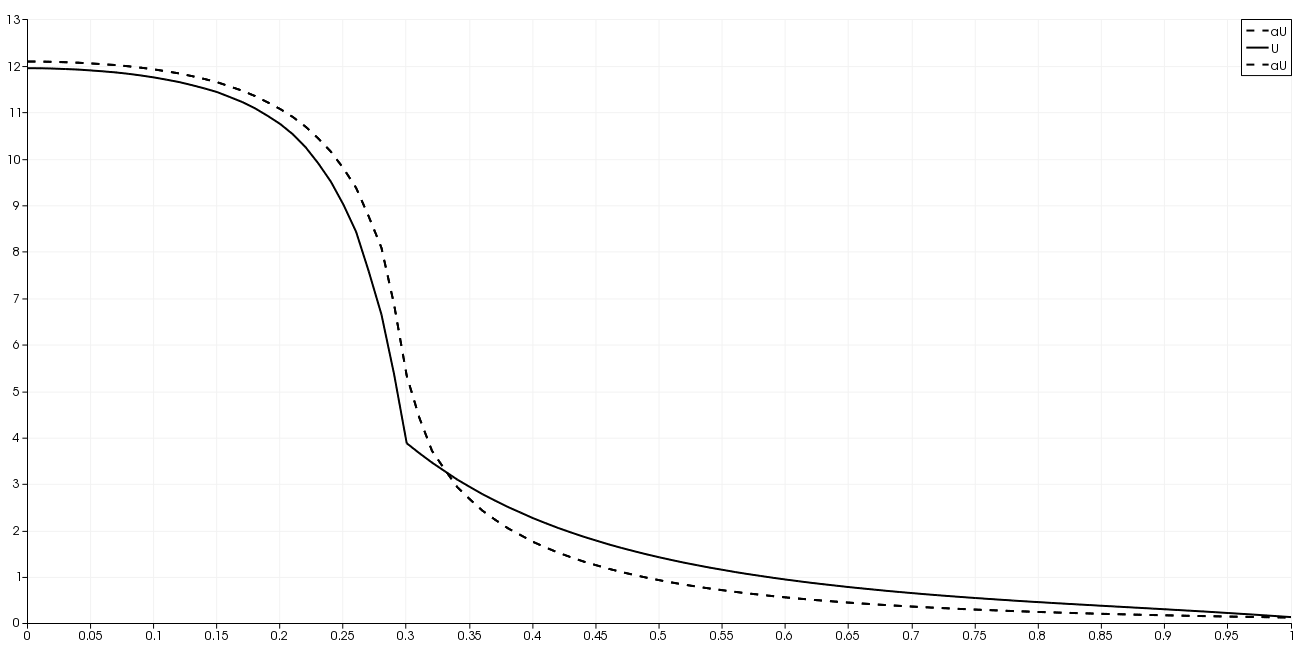
\includegraphics[height=0.5\textheight]{n2}}%
	\only<3>{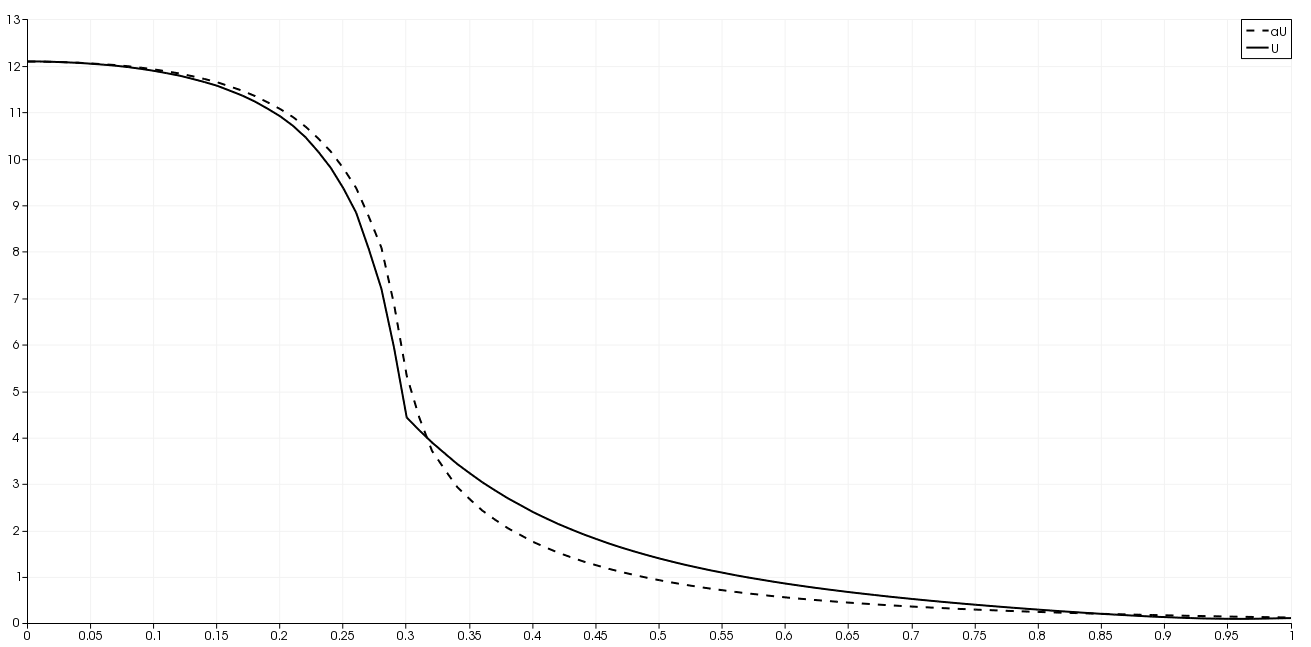
\includegraphics[height=0.5\textheight]{n3}}%
	\only<4>{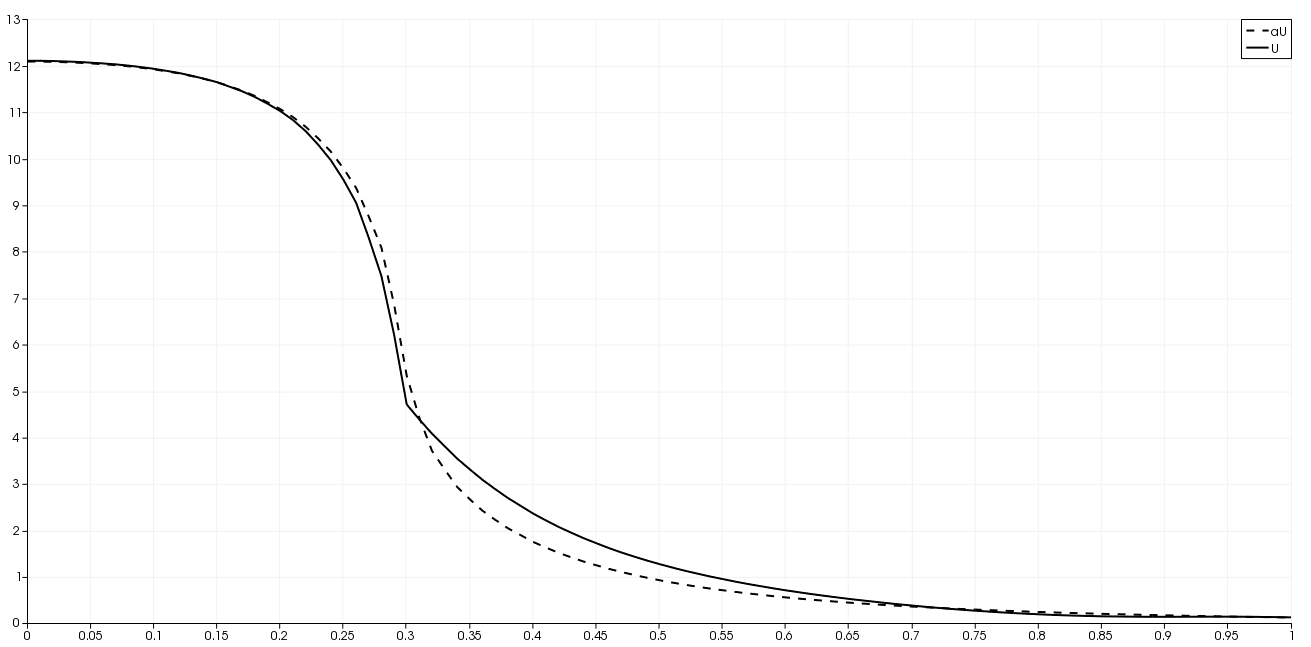
\includegraphics[height=0.5\textheight]{n4}}%
	\only<5>{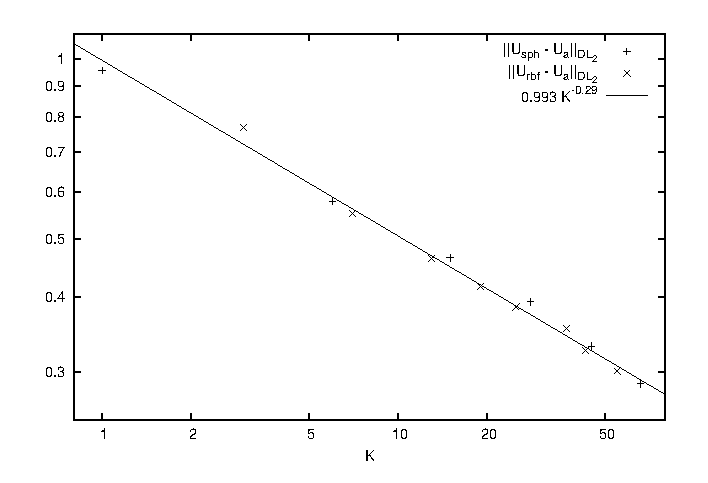
\includegraphics[height=0.5\textheight]{UL2err.eps}}

    \only<1>{$K = 1$}%
    \only<2>{$K = 6$}%
    \only<3>{$K = 15$}%
    \only<4>{$K = 28$}%
	\only<5>{Порядок сходимости $\varepsilon_{L_2} \sim K^{-0.29}$}
\end{center}
\end{frame}

\begin{frame}\frametitle{Сходимость внешних итераций (МСГ)}
\begin{table}[ht!]
\centering
\caption{Количество итераций метода сопряженных градиентов}
\begin{tabular}{cc|c|c|c|c|c|c|}
\cline{3-8}
& & \multicolumn{6}{|c|}{\rule{0em}{2.2ex}Количество узлов сетки} \\ \cline{3-8}
& & \rule{0em}{2.2ex}6996 & 12971 & 26786 & 53109 & 99015 & 205756\\ \cline{1-8}
\multicolumn{1}{|c|}{\multirow{7}{*}{\rotatebox{90}{Угловых
гармоник\phantom{x}}}} &
\multicolumn{1}{|c|}{\rule{0em}{2.2ex}1}  & 1 & 1 & 1 & 1 & 1 & 1 \\ 
\cline{2-8}\multicolumn{1}{|c|}{} &
\multicolumn{1}{|c|}{\rule{0em}{2.2ex}6}  & 20 & 21 & 22 & 23 & 25 & 26 \\ 
\cline{2-8}\multicolumn{1}{|c|}{} &
\multicolumn{1}{|c|}{\rule{0em}{2.2ex}15} & 29 & 31 & 33 & 34 & 37 & 38 \\ 
\cline{2-8}\multicolumn{1}{|c|}{} &
\multicolumn{1}{|c|}{\rule{0em}{2.2ex}28} & 36 & 38 & 41 & 44 & 48 & 51 \\ 
\cline{2-8}\multicolumn{1}{|c|}{} &
\multicolumn{1}{|c|}{\rule{0em}{2.2ex}45} & 42 & 45 & 49 & 53 & 57 & 62 \\ 
\cline{2-8}\multicolumn{1}{|c|}{} &
\multicolumn{1}{|c|}{\rule{0em}{2.2ex}66} & 46 & 50 & 55 & 60 & 65 & 70 \\ 
\cline{2-8}\multicolumn{1}{|c|}{} &
\multicolumn{1}{|c|}{\rule{0em}{2.2ex}91} & 48 & 53 & 59 & 65 & 71 & 77 \\ 
\cline{1-8}
\end{tabular}
\end{table}

Число итераций до сходимости зависит как от числа угловых функций $K$, так и от
числа узлов сетки $N$.

\end{frame}

\begin{frame}\frametitle{Сходимость внешних итераций (МСГ)}
\begin{table}[ht!]
\centering
\caption{Количество итераций метода с радиальным базисом}
\begin{tabular}{cc|c|c|c|c|c|c|}
\cline{3-8}
& & \multicolumn{6}{|c|}{\rule{0em}{2.2ex}Количество узлов сетки} \\ \cline{3-8}
& & \rule{0em}{2.2ex}6996 & 12971 & 26786 & 53109 & 99015 & 205756\\ \cline{1-8}
\multicolumn{1}{|c|}{\multirow{7}{*}{\rotatebox{90}{Угловых
гармоник\phantom{x}}}} &
\multicolumn{1}{|c|}{\rule{0em}{2.2ex}3}  & 13 & 14 & 15 & 14 & 15 & 15 \\ 
\cline{2-8}\multicolumn{1}{|c|}{} &
\multicolumn{1}{|c|}{\rule{0em}{2.2ex}7}  & 26 & 27 & 28 & 28 & 29 & 31 \\ 
\cline{2-8}\multicolumn{1}{|c|}{} &
\multicolumn{1}{|c|}{\rule{0em}{2.2ex}13} & 33 & 34 & 35 & 36 & 39 & 42 \\ 
\cline{2-8}\multicolumn{1}{|c|}{} &
\multicolumn{1}{|c|}{\rule{0em}{2.2ex}19} & 26 & 28 & 29 & 29 & 30 & 32 \\ 
\cline{2-8}\multicolumn{1}{|c|}{} &
\multicolumn{1}{|c|}{\rule{0em}{2.2ex}25} & 28 & 29 & 32 & 30 & 32 & 34 \\ 
\cline{2-8}\multicolumn{1}{|c|}{} &
\multicolumn{1}{|c|}{\rule{0em}{2.2ex}43} & 28 & 30 & 32 & 31 & 33 & 34 \\ 
\cline{2-8}\multicolumn{1}{|c|}{} &
\multicolumn{1}{|c|}{\rule{0em}{2.2ex}55} & 27 & 28 & 30 & 29 & 30 & 32 \\ 
\cline{1-8}
\end{tabular}
\end{table}

Число итераций до сходимости практически не зависит от числа угловых функций
$K$.

\end{frame}


\begin{frame}\frametitle{Выводы}
	\begin{itemize}
	\item Скорость сходимости в норме $L_2$ зависит лишь от числа угловых
функций, а не от их типа.
	\item Оба метода испытывают затруднения в области перехода из оптически плотной среды в оптически тонкую.
	\item Предложенный метод с радиальными базисными функциями сходится быстрее
метода сферических функций при $K > 15$.
	\end{itemize}
\end{frame}

% ===========================================================

\section{Маршевый метод коротких характеристик}
\subsection{Метод коротких характеристик}
\begin{frame}\frametitle{Метод коротких характеристик}
	\begin{itemize}
	\item Метод коротких характеристик основан на идее сеточно-характеристического метода. Из каждого узла расчетной сетки выпускается характеристика вдоль направления $-\vec \Omega$ до пересечения с ближайшей гранью.
	
	\item При этом решение в узле находится по формуле
	\[
	\I(\vec r) = \I_\text{p} (1 - e^{-\tau}) + \I^* e^{-\tau}, \qquad
	\tau = \varkappa ||\vec r - \vec r^*|| 
	\]
	\end{itemize}
	\begin{figure}
	\centering
	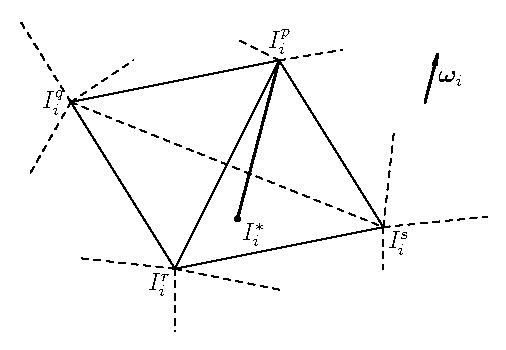
\includegraphics[height=.35\textheight]{radiation-2.eps}
	\caption{Характеристика уравнения переноса}
	\end{figure}
\end{frame}

\subsection{Маршевый алгоритм}
\begin{frame}\frametitle{Маршевый алгоритм}
	\begin{itemize}
	\item Решение в тетраэдре можно находить только после того, как найдено
решения во всех тетраэдрах, граничащих по входным граням. Данное условие задает порядок обхода тетраэдров сетки.
	\item Для триангуляций Делоне данный порядок соответствует порядку проекций
центров описанных сфер тетраэдров на направление $\vec \Omega$.
	\item Для произвольных триангуляций используется алгоритм топологической
сортировки Тарьяна. При этом множество тетраэдров разбивается на независимые
ярусы. Решения в тетраэдрах из одного яруса независимы и их можно находить
параллельно.
	\end{itemize}
	\begin{center}
	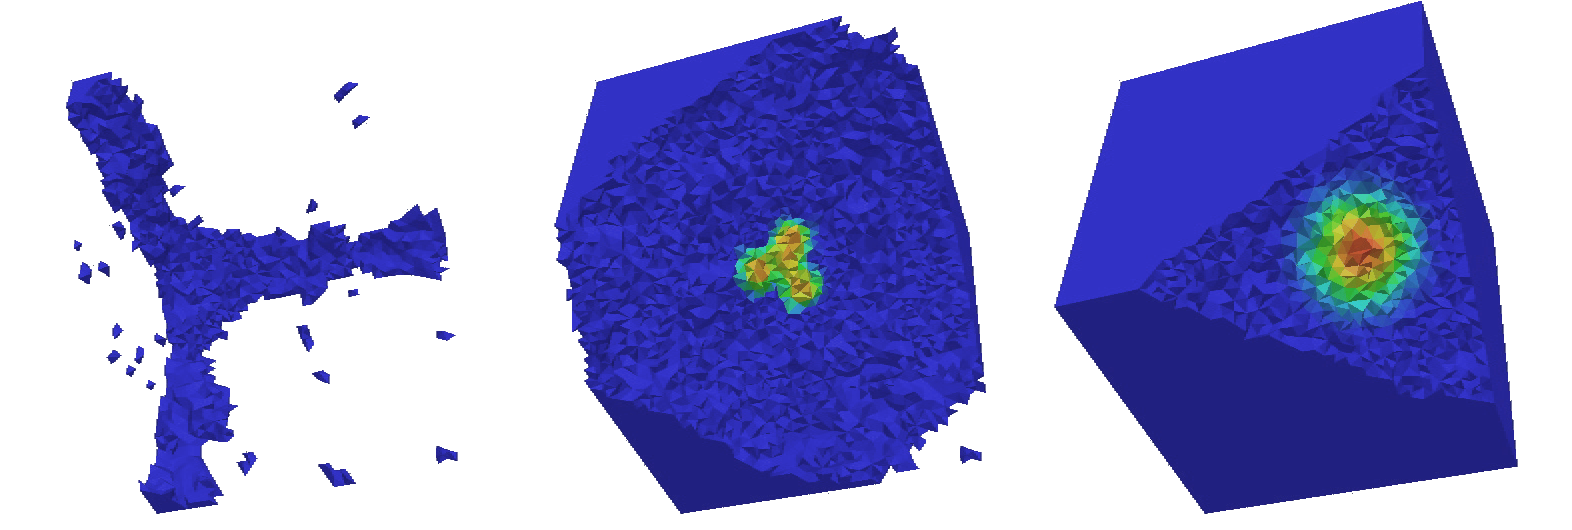
\includegraphics[height=.3\textheight]{123.png}
	\end{center}
\end{frame}

\subsection{Повышение порядка}
\begin{frame}\frametitle{Метод второго порядка}
	\begin{itemize}
	\item Для повышения порядка аппроксимации метода в тетраэдрах выбираются
дополнительные узлы на ребрах.
	\item При этом не меняется маршевый порядок обхода тетраэдров.
	\item Для монотонизации схемы использован ограничитель решения в дополнительных узлах.
	\end{itemize}

	\[
	\tilde \I_\text{mid} = \frac{\I_1 + \I_2}{2} + \max\left(\frac{-|\I_2 - \I_1|}{4},
	\min\left(
	\frac{|\I_2 - \I_1|}{4},
	\I_\text{mid} - \frac{\I_1 + \I_2}{2}
	\right)
	\right)
	\]
	
	\begin{figure}
	\centering
	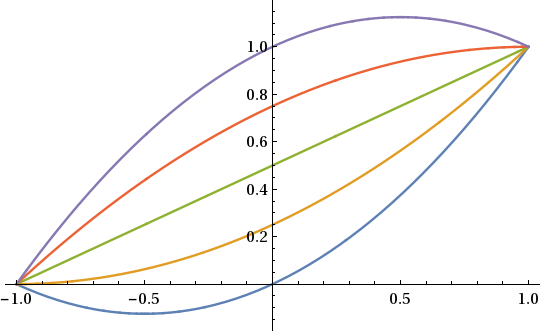
\includegraphics[height=.3\textheight]{mono.png}
	\end{figure}	
\end{frame}

\begin{frame}\frametitle{Сравнение методов}

	\begin{itemize}
	\item Метод второго порядка без ограничителя имеет нефизические осцилляции на уровне $20 \%$.
	\item Метод с ограничителем обладает существенно меньшей схемной диффузией, чем метод первого порядка.
	\end{itemize}

	\begin{figure}
	\centering
	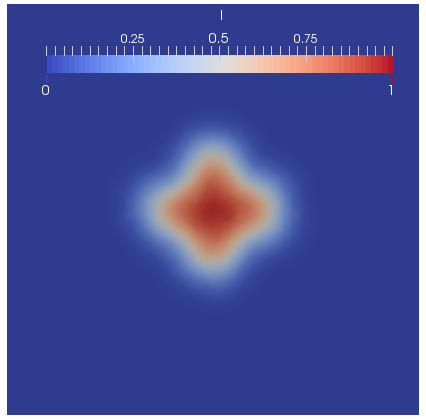
\includegraphics[width=.3\textwidth]{res1ord.png} %
	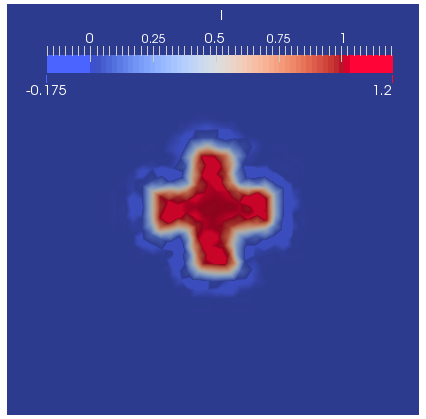
\includegraphics[width=.3\textwidth]{res2nolim.png} %
	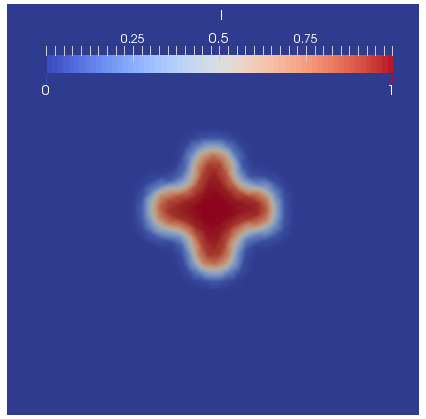
\includegraphics[width=.3\textwidth]{res2wilim.png} %
	\caption{Решения вдоль направления к наблюдателю, полученные методами первого порядка, второго порядка и второго порядка с ограничителем}
	\end{figure}
\end{frame}

\subsection{Выводы}
\begin{frame}\frametitle{Выводы}
	\begin{itemize}
	\item Предложен маршевый алгоритм, который может быть применен не только для метода коротких характеристик, но и для других методов решения стационарных гиперболических задач.
	\item Алгоритм строит ярусно-параллельную форму метода, которая может быть использована для построения параллельной версии алгоритма.
	\item Построен метод второго порядка и его монотонный вариант.
	\end{itemize}
\end{frame}

% ===========================================================

\section{Распределенный метод длинных характеристик}
\subsection{Метод длинных характеристик}

\begin{frame}\frametitle{Метод длинных характеристик}
	\begin{itemize}
	\item Уравнение переноса излучения имеет гиперболический тип и семейство
характеристик вида
	\[
		\vec x - \vec x_0 = \vec \Omega s, \qquad s > 0.
	\]
	\item Вдоль характеристик уравнение тривиально интегрируется:
	\[
		\I(\vec x, \vec \Omega) = \alpha(0, s) \I(\vec x_0, \vec \Omega) + \beta(0, s),
	\]
	где
	\[
		\alpha(s_0, s) = \exp\left\{-\int_{s_0}^s \varkappa(\zeta) d\zeta\right\}
		\qquad
		\beta(s_0, s) = \int_{s_0}^s \varkappa(\xi) \Ip(\xi) \alpha(\xi, s) d\xi.
	\]
	\item Из каждой точки $\vec x$ выпускается набор характеристик в
направлениях $\vec \omega_i$ до
пересечения с границей области, где используется граничное условие.
	\end{itemize}
\end{frame}

\subsection{Предлагаемый подход}
\begin{frame}\frametitle{Распределенный метод}
	\begin{itemize}
	\item В случае, когда характеристики выпускаются не до границей
области, получаются линейные соотношения, связывающие
интенсивности в двух точках --- $\vec x$ и $\vec x_0$
\[
\I(\vec x, \vec \Omega) = \alpha(0, s) \I(\vec x_0, \vec \Omega) + \beta(0, s),
\qquad \vec x - \vec x_0 = \vec \Omega s.
\]
	\item Выпустив по характеристике из каждой точки, как с границы области, так
и с границ подобластей, можно получить небольшую систему линейных уравнений,
куда входят только значения интенсивности на границах расчетных подобластей.

	\item После того как граничные значения в каждой подобласти найдены, значения
внутри могут быть найдены автономно от других подобластей.
	\end{itemize}
\end{frame}

\begin{frame}\frametitle{Последовательный и распределенный метод}
	\begin{figure}
	\centering
	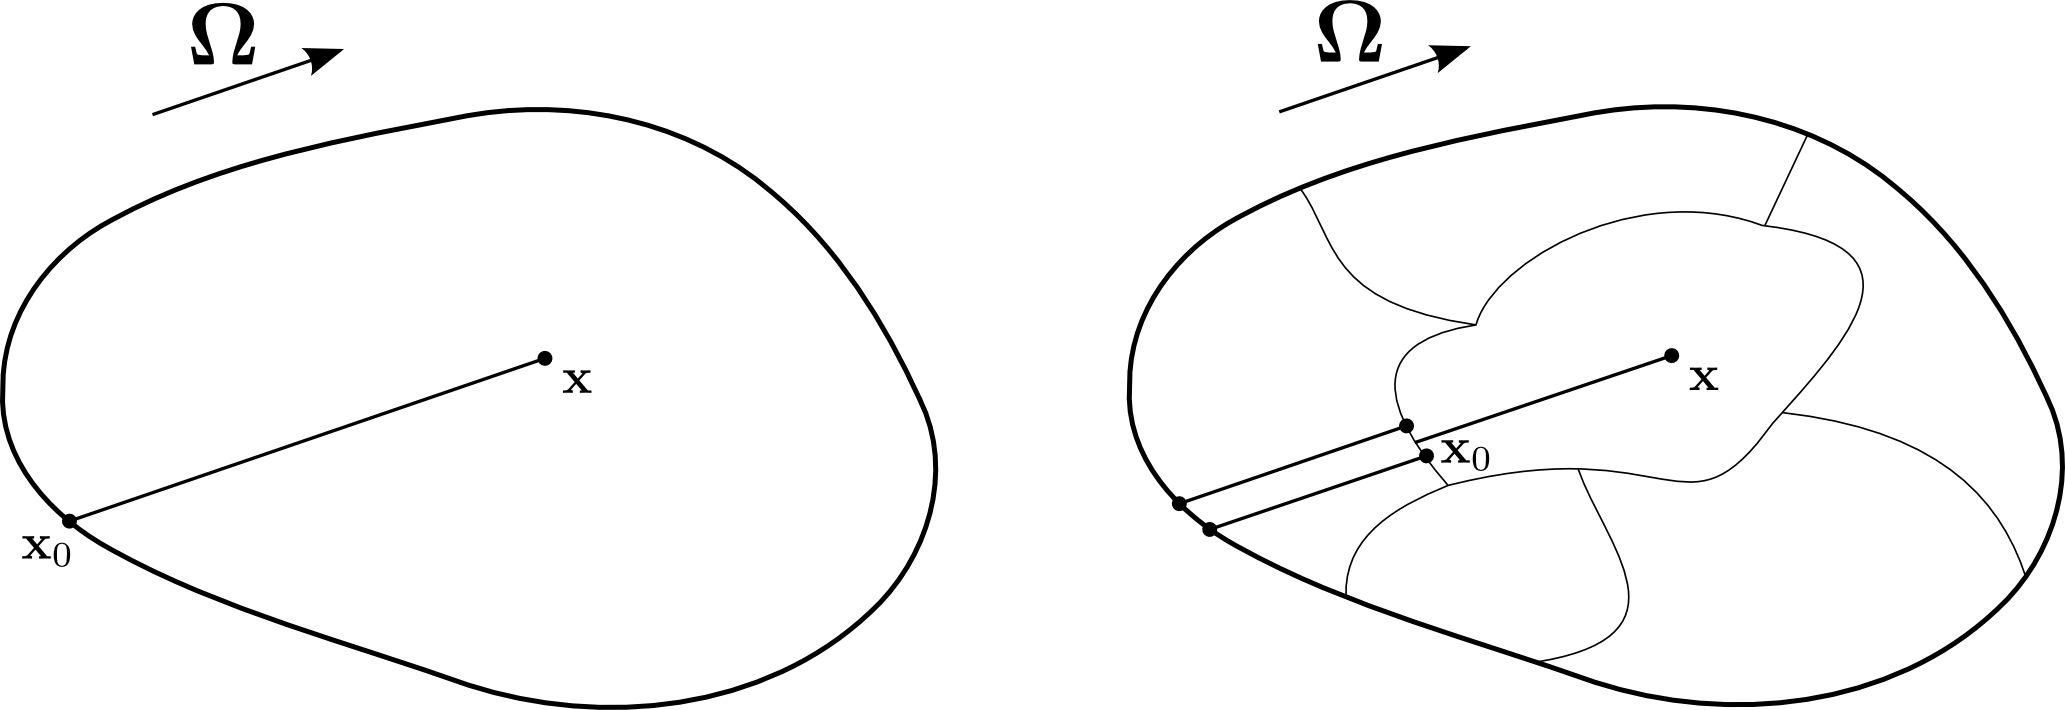
\includegraphics[height=.4\textheight]{methods.png}
	\caption{Трассировка во всей области и в отдельной подобласти}
	\end{figure}
\end{frame}

\subsection{Алгоритмическая реализация}
\begin{frame}\frametitle{Алгоритм решения}
	Для каждого из направлений квадратурной формулы повторяются шаги:
	\begin{itemize}
	\item Граничные вершины каждой подобласти разбиваются на входные и выходные
по отношению к направлению характеристики.
	\item Из каждой выходной вершины производится трассировка подобласти.
Трассировка заканчивается на грани с входными вершинами.
	\item На одном из вычислительных процессов собирается система уравнений и
решается прямым методом. Такой выбор обусловлен преимущественно треугольной
формой матрицы. Полученное решение рассылается подобластям.
	\item После этого в каждой подобласти автономно производится трассировка из
каждой вершины. Это самая длительная операция.
	\end{itemize}
\end{frame}

\begin{frame}\frametitle{Особенности реализации алгоритма}
	\begin{itemize}
	\item Для балансировки загрузки, обработка направлений производится по
несколько за раз. Это увеличивает время подготовительного этапа, но позволят
решать линейные системы от разных направлений одновременно.
	\item Последний (автономный) этап реализован с использованием графических
ускорителей (GPU).
	\item Благодаря асинхронному режиму работы GPU, удается
произвести перекрытие расчета на GPU с подготовительным этапом на CPU для
следующего набора направлений.
	\begin{center}
	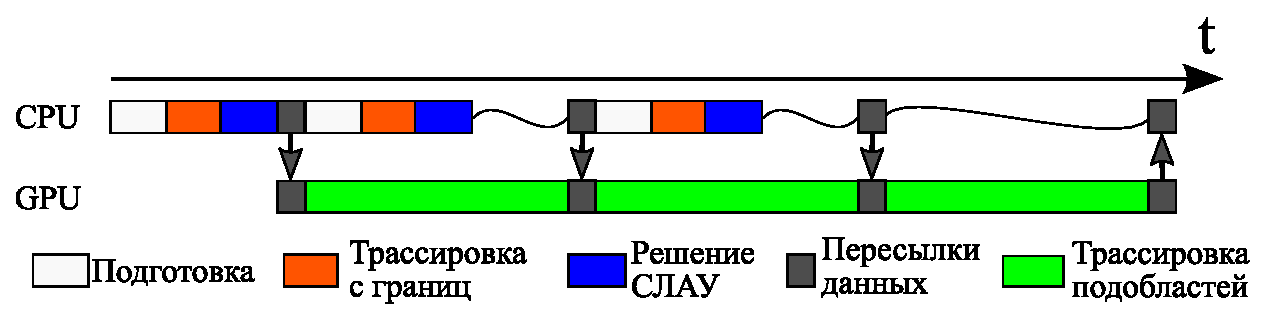
\includegraphics[height=.25\textheight]{timeline.eps}
	\end{center}
	\end{itemize}
\end{frame}

\subsection{Результаты}
\begin{frame}\frametitle{Диффузия на границах областей}
	Метод имеет незначительную численную диффузию луча, который проходит вблизи
поверхности раздела подобластей. При суммировании по различным направлениям этот
эффект становится менее заметен.
	\begin{figure}
	\centering
	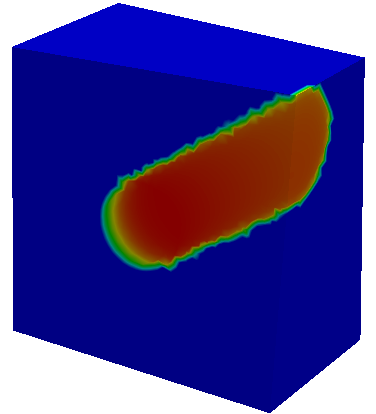
\includegraphics[height=.4\textheight]{res1piece.png}
	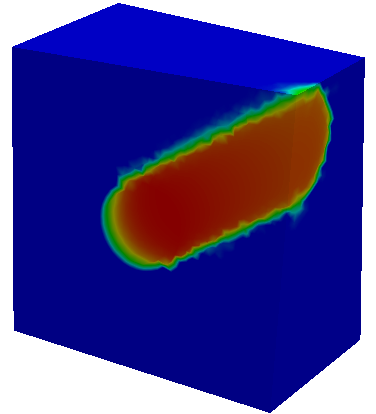
\includegraphics[height=.4\textheight]{res8pieces.png}
	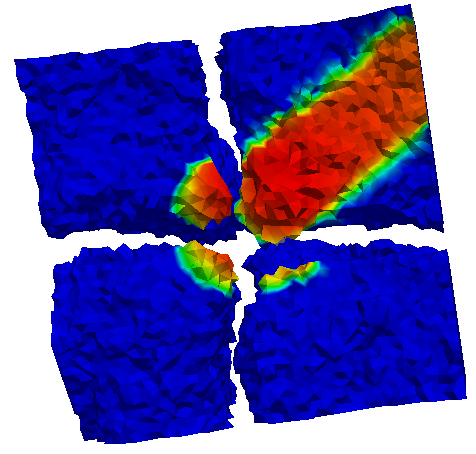
\includegraphics[height=.4\textheight]{ressplit.png}
	\caption{Численная диффузия луча, идущего вдоль границы раздела областей}
	\end{figure}
\end{frame}

\begin{frame}\frametitle{Ускорение}
	Для тестов использовалась тетраэдральная сетка из $65.8 \cdot 10^3$ узлов
($363\cdot10^3$ тетраэдров) и квадратурная формула Лебедева $25$-го порядка
($230$
направлений)
	\begin{table}
	\begin{tabular}{|c|c|c|c|c|}
	\hline
	$P$ & Устройства & $t_\text{GPU}, \text{c}$ & $t_\text{CPU}, \text{c}$ & $t_\text{CPU} / t_\text{GPU}$\\\hline
	$1$& 1 x Tesla C2075 & $117$ & $439$ & $3.75$x\\\hline
	$2$& 2 x Tesla C2075 & $52$ & $196$ & $3.77$x\\\hline
	$3$& 3 x Tesla C2075 & $32.7$ & $125$ & $3.82$x\\\hline
	$4$& 3 x Tesla C2075 + GTX 680 & $28.1$ & $108$ & $3.84$x\\
%	$4$& 1 x Tesla C2075 & $88$ & $108$ & $1.23$x\\
\hline
	$8$& 3 x Tesla C2075 + GTX 680 & $25.5$ & $69$ & $2.70$x\\\hline
	\end{tabular}
	\caption{Сравнительные времена работы алгоритма}
	\end{table}
\end{frame}

\begin{frame}\frametitle{Изоповерхности решения}
	Для данной задачи при $230$ направлениях на изоповерхностях плотности
энергии излучения можно наблюдать небольшие искажения в направлениях $\pm x, \pm y, \pm
z$.
	\begin{figure}
	\centering
	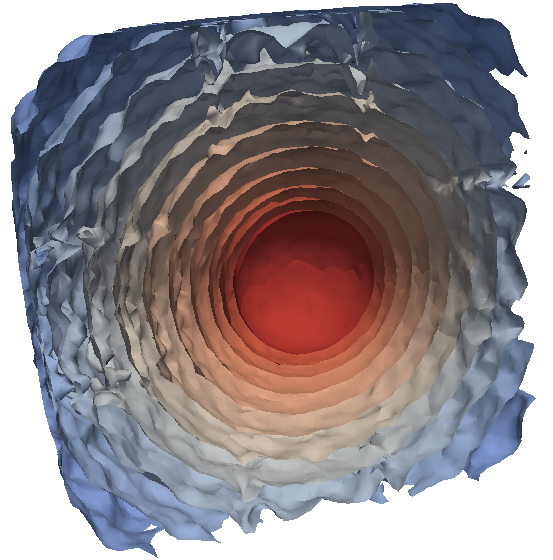
\includegraphics[height=.6\textheight]{isomcm.png}
	\end{figure}
\end{frame}

\begin{frame}\frametitle{Выводы}
	\begin{itemize}
	\item GPU реализация данного алгоритма оказалась малоэффективной. В
значительной степени это обусловлено хаотичным доступом к памяти, происходящим
при трассировке сетки.
	\item Решения по каждому направлению получаются очень точными. В свою
очередь, это также вызывает <<эффект луча>> и требует подробной сетки
направлений.
	\item Суммарная вычислительная стоимость метода на порядки превосходит 
	вычислительную стоимость методов семейства коротких характеристик.
	\end{itemize}
\end{frame}

\section{Спектр линии H-$\alpha$ звезды}

\subsection{Постановка задачи}
\begin{frame}\frametitle{Постановка задачи}
\begin{itemize}
\item
Для имеющихся результатов МГД моделирования взаимодействия акреционного диска со звездой типа Т Тельца необходимо построить наблюдаемый с Земли спектр излучения в окрестности линии H-$\alpha$. При этом учитывается доплеровский сдвиг частоты поглощения вещества.
\item Коэффициент поглощения был вычислен в предположении, что окружающее звезду
вещество состоит из атомов H и ионов H$^{+}$.
\end{itemize}
\begin{figure}[ht!]
\centering
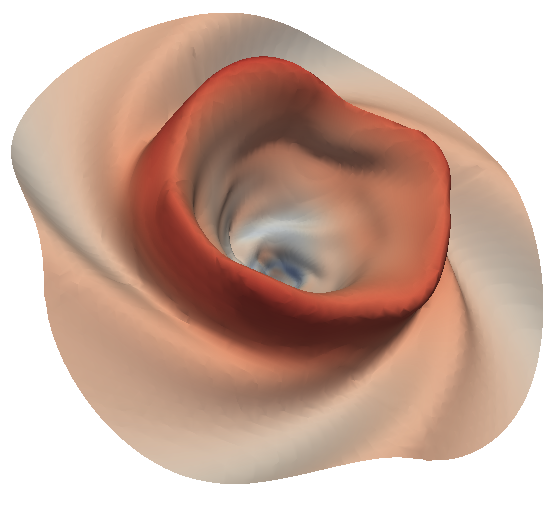
\includegraphics[height=3cm]{wind.png}
\caption{Изоповерхность плотности вещества, окружающего звезду}
\end{figure}
\end{frame}

\subsection{Результаты}

\begin{frame}\frametitle{Интенсивность излучения в различных направлениях}
\begin{columns}\begin{column}{.6\textwidth}
\begin{itemize}
\item Средний за оборот звезды поток излучения от звезды находился одновременно
для разных ориентаций плоскости диска. Для этого используется специальная сетка,
равномерная по углам $\theta, \varphi$.
\item Профиль линии разбивается на $64$ частотные группы, соответствующие
доплеровскому смещению до $\pm 600 \text{ км}/\text{с}$
\end{itemize}
\end{column}\begin{column}{.4\textwidth}
\begin{figure}[ht!]
\centering
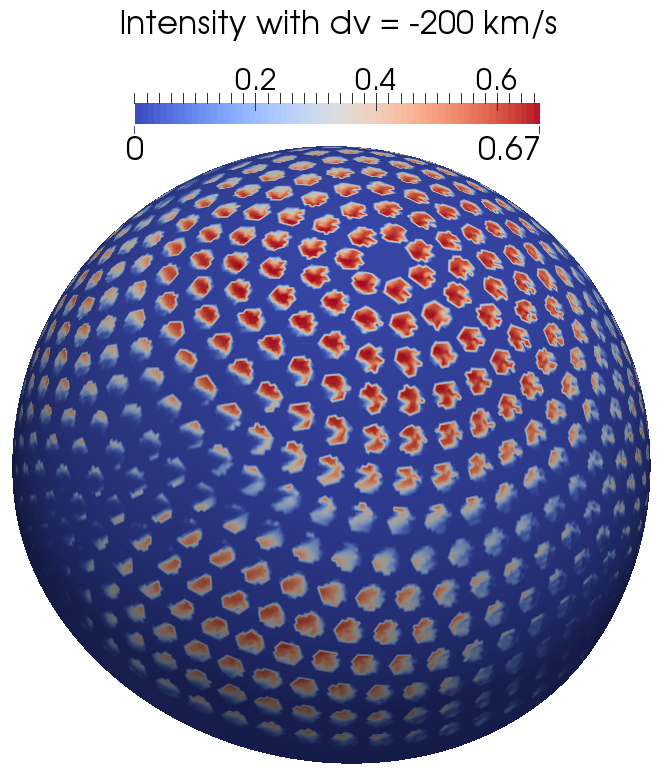
\includegraphics[height=.5\textheight]{trace.png} %
\caption{Излучение в различных направлениях в частотной группе, соответствующей синему
смещению в $200 \text{ км}/\text{с}$}
\end{figure}
\end{column}\end{columns}
\end{frame}

\begin{frame}\frametitle{Спектр}
Нормализованный профиль линии излучения имеет существенный провал в области
красного смещения на скорости $\Delta v \approx 100 \text{ км}/\text{с}$, который объясняется значительным поглощением излучения веществом диска, аккрецирующего на звезду.
\begin{figure}[ht!]
\centering
%\includegraphics[width=.45\textwidth]{varinc.eps} %
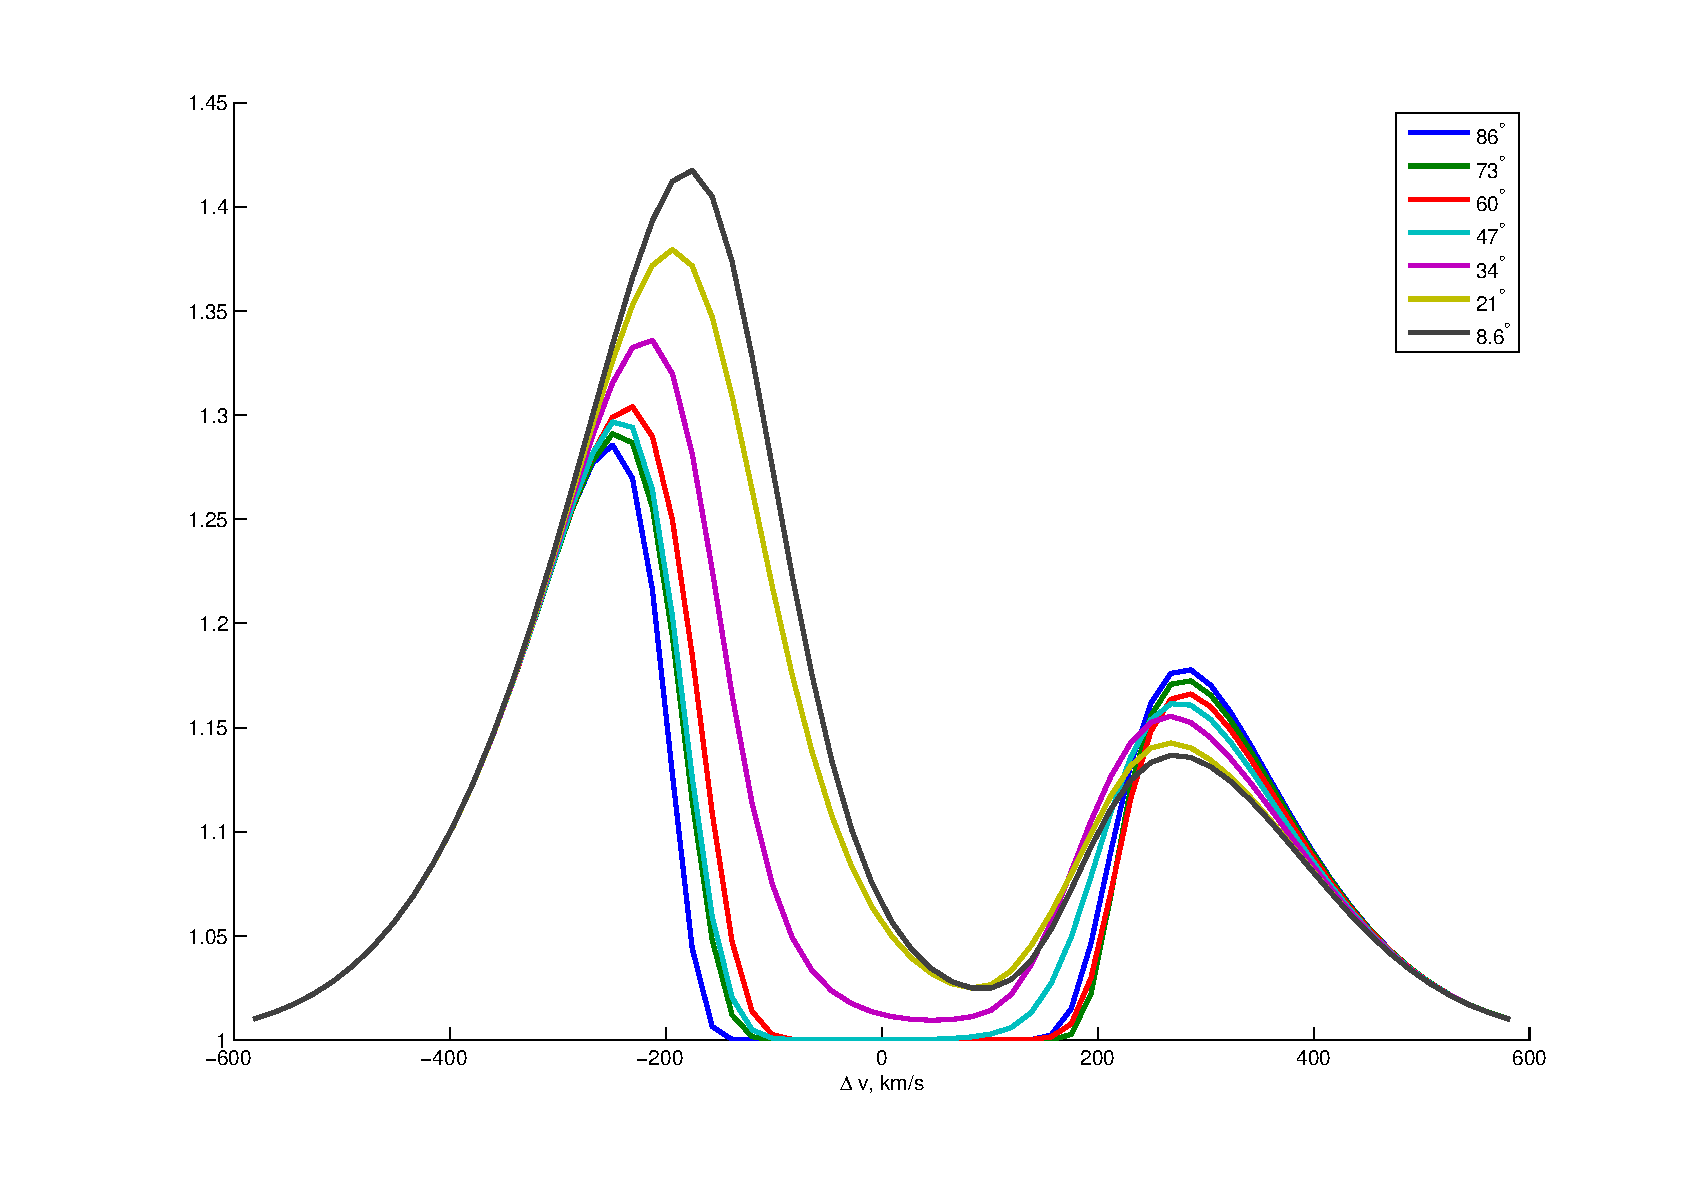
\includegraphics[height=.62\textheight]{spectrum.eps} %
\caption{Нормализованный профиль линии H-$\alpha$ в зависимости от угла наклонения $i$}
\end{figure}	
\end{frame}

\section{Заключение}
\subsection{Основные результаты диссертации}
\begin{frame}\frametitle{Основные результаты 1/3}
\begin{itemize}
  \item Для решения уравнения переноса излучения разработан вариационный метод с
радиальными базисными функциями, который обладает точностью, сравнимой с
точностью метода сферических гармоник, но при этом является более экономичным.
Экономичность была достигнута за счет использования предложенного блочно-диагонального 
предобуславливания метода решения системы линейных уравнений. 
  \item Разработан маршевый метод коротких характеристик. Построены варианты
данного метода первого и второго порядка аппроксимации. Получено условие
расположения узлов, выполнение которого необходимо для устойчивости метода
второго порядка. Для монотонизации схемы второго порядка применен ограничитель
значения интенсивности в дополнительных узлах.
\end{itemize}
\end{frame}

\begin{frame}\frametitle{Основные результаты 2/3}
\begin{itemize}
  \item Для маршевого метода построены алгоритмы упорядочения
неструктурированных сеток. Дополнительным результатом работы алгоритмов
упорядочения является ярусно-параллельная форма графа зависимостей
вычислительного метода, которую можно использовать для распараллеливания
процесса решения задачи. 
  \item Разработана версия метода длинных характеристик, адаптированная для
распределенной реализации на многопроцессорных системах и на кластерах с
графическими ускорителями. Исследованы ускорение и эффективность реализаций
метода в зависимости от числа используемых вычислительных узлов и графических
ускорителей.
\end{itemize}
\end{frame}

\begin{frame}\frametitle{Основные результаты 3/3}
\begin{itemize}
  \item Разработанные вычислительные алгоритмы реализованы в виде программного
комплекса. В рамках модели локального термодинамического равновесия вычислен
коэффициент поглощения частично ионизованной плазмы. Для задачи моделирования
спектра излучения звезды типа Т Тельца построен спектральный профиль линии
H-$\alpha$ в зависимости от ориентации плоскости аккреционного диска.
\end{itemize}
\end{frame}

\begin{frame}[plain]
  \begin{center}
  {\Huge Спасибо за внимание!}
  \vspace{8ex}

  Цыбулин Иван

  e-mail: \colorhref{mailto:tsybulin@crec.mipt.ru}{tsybulin@crec.mipt.ru}
  \end{center}
\end{frame}

\begin{frame}[allowframebreaks]\frametitle{Публикации автора по теме диссертации}
\nocite{*}
\tiny
\insertbiblioauthor
\end{frame}

\end{document}
